\section{Rotatore rigido}
Come esempio di sistema quantomeccanico molto semplice si vuole studiare in questo capitolo il \emph{rotatore rigido unidimensionale}. Un sistema di questo tipo è caratterizzato da un angolo di rotazione $\varphi$ che varia tra $0$ e $2\pi$. 
\begin{figure}[H]
    \centering
    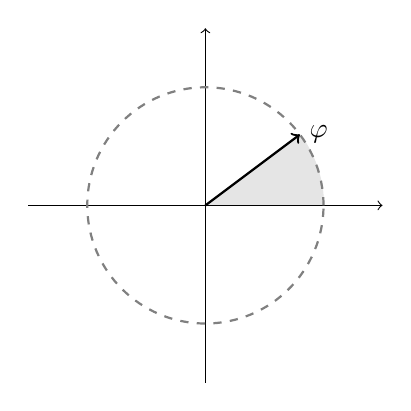
\begin{tikzpicture}[scale=1.5]
        \draw[fill=black!10,black!10] (0,0) -- (1,0) arc(0:36.8698976:1)node[anchor=west,black]{$\varphi$} (.8,.6) -- (0,0);
        \draw[->] (0,-1.5) -- (0,1.5);
        \draw[->] (-1.5,0) -- (1.5,0);
        \draw[dashed,color=gray,thick] (0,0) circle (1);
        \draw[->,thick] (0,0) -- (.8,.6);
    \end{tikzpicture}
\end{figure}
Classicamente ad un angolo di rotazione è associato un momento generalizzato $P_\varphi$. Analogamente in meccanica quantistica s vogliono definire gli operatori autoaggiunti $\hat \varphi$ e $\hat P_\varphi$. Per prima cosa, utilizzando il principio di quantizzazione, si deve imporre la relazione di commutazione imposta dalle parentesi di Poisson classiche:
\begin{equation*}
    \{\varphi,P_\varphi\}=1\qquad\Rightarrow\qquad[\hat\varphi,\hat P_\varphi]=i\hslash\hat{I}.
\end{equation*}
Si vuole che $\hat\varphi$ di origine ad una base di autoket ortonormale che si indicherà con $\ket{\varphi}$. Lo spettro di questo operatore è continuo (siccome deve rappresentare un angolo nello spazio delle configurazioni) e si suppone che valgano le seguenti relazioni (in analogia con quanto accade con $x$ nella rappresentazione di Schrödinger):
\begin{equation*}
    \bra{\varphi}\hat\varphi=\varphi\bra{\varphi},\qquad\bra{\varphi}\hat P_\varphi=-i\hslash\frac{d}{d\phi}\bra{\varphi}.
\end{equation*}
Siccome $\varphi$ rappresenta un angolo si vuole che una rotazione di $2\pi$ non modifichi lo stato del sistema ($\ket{\varphi+2\pi}=\ket{\varphi}$), questa richiesta però non è compatibile con le relazioni agli autovalori precedenti. Per questo motivo il dominio dello spettro è ristretto in $[-\pi,\pi]$. Varranno quindi le seguenti relazioni di completezza:
\begin{equation*}
    \braket{\varphi'|\varphi}=\sum_{k=\infty}^{\infty}\delta(\varphi'-\varphi+2\pi k),\qquad\int_{-\pi}^{+\pi}\ket{\varphi}d\varphi\bra{\varphi}=\hat I,
\end{equation*}
In questo modo $\varphi$ da origine ad una rappresentazione "angolare".
dove $\delta(x)$ è la delta di Dirac.
\subsection{Spettro dell'operatore momento}
Si vuole ora studiare lo spettro dell'operatore $\hat P_\varphi$. Se si suppone $\ket{p_\varphi}$ autoket di $\hat P_\varphi$ si ha:
\begin{equation*}
    \hat P_\varphi\ket{\hat P_\varphi}=\ket{\hat P_\varphi}\hat P_\varphi.
\end{equation*}
Utilizzando la rappresentazione che si è appena creata si ha:
\begin{equation*}
    \bra{\varphi}\hat P_\varphi\ket{\hat P_\varphi}=-i\hslash\frac{d}{d\phi}\braket{\varphi|P_\varphi}=\braket{\varphi|P_\varphi}P_\varphi.
\end{equation*}
Questa è di fatto un'equazione differenziale per $\braket{\varphi|P_\varphi}$ che risulta quindi:
\begin{equation*}
    \braket{\varphi|P_\varphi}=ce^{\frac{i}{\hslash}P_\varphi\varphi},
\end{equation*}
dove $c$ è una costante complessa da determinare imponendo la normalizazione degli autoket.\\
A questo punto è necessario imporre le condizioni di periodicità richiesta dalla natura angolare di $\varphi$:
\begin{equation*}
    \braket{\varphi+2\pi|P_\varphi}=\braket{\varphi|P_\varphi}\quad\Rightarrow\quad e^{\frac{i}{\hslash}2\pi P_\varphi}=1\quad\Rightarrow\quad\frac{i}{\hslash}2\pi P_\varphi=2m\pi i,\ m\in\mathbb{Z}\quad\Rightarrow\quad P_\varphi=\hslash m,\ m\in\mathbb{Z}.
\end{equation*}
\begin{proposition}
    L'operatore $\hat P_\varphi$ ha spettro discreto dato da $\{\dots,-2\hslash,-\hslash,0,\hslash,2\hslash,\dots\}$.
\end{proposition}
In questo modo la base di autoket di $\hat P_\varphi$ è rinominato:
\begin{equation*}
    \hat P_\varphi\ket{m}=\ket{m}\hslash m,\qquad\braket{\varphi|m}=\frac{e^{im\varphi}}{\sqrt{2\pi}}.
\end{equation*}